% Chapter 3
% 
\chapter{Planning} % Main chapter title

%-------------------------------------------------------------------------------
%---------

This chapter serves to outline the planning aspects of the project. It begins with the definition of the Project Charter, where it is defined the important aspects of the project, marking it as the starting point. After this is defined, the \gls{WBS} is defined, leading to an overall view of the project. For the last one a Gantt diagram is presented detailing in a more fine-grand aspects all the tasks necessary to the project.

\section{Project Charter}

The project charter provides a comprehensive overview of the project scope, stakeholders, benefits, assumptions, and restrictions.

\noindent \textbf{Stakeholder}

\begin{table}[h!]
    \centering
    \begin{tabular}{|p{11cm}|c|c|}
        \hline
        \textbf{Identification}                                                         & \textbf{Power} & \textbf{Interest} \\ \hline
        External reviewers who may evaluate the dissertation                            & Low            & Low               \\ \hline
        Students or developers in the areas of distributed systems and fault tolerance  & Low            & Low               \\ \hline
        Administration of the master's program, responsible for dissertation evaluation & Medium         & Low               \\ \hline
        Supervisor (advisor)                                                            & High           & High              \\ \hline
    \end{tabular}
\end{table}

The external reviewers and developers represent an indirect audience with limited direct influence but potential interest in the outcomes. The master's program administration has moderate influence due to institutional requirements, while the supervisor holds the most significant influence and interest, as their guidance and approval are critical for project success.

\textbf{Benefits}

\begin{itemize}
    \item \textbf{Decision Support for Developers:}
          The project will provide a detailed analysis of fault tolerance aspects in Elixir, Go, and Scala with Akka, offering developers and system architects a practical guide to help them choose the most suitable language for specific fault-tolerant distributed systems scenarios.

    \item \textbf{Open Source Opportunities:}
          The findings could reveal areas for improvement in the evaluated languages, inspiring open-source developers to create libraries, frameworks, or enhancements tailored to fault tolerance in distributed environments.

    \item \textbf{Academic Contributions:}
          The dissertation will contribute to the existing body of knowledge in the areas of distributed systems, fault tolerance, and microservices. It will provide insights into comparative aspects in the languages of debate..

\end{itemize}

\noindent \textbf{Assumptions}

\begin{itemize}
    \item \textbf{Computational Resources:}
          It is assumed that the available computational resources, including hardware and software tools, will suffice to simulate the benchmarking scenarios for each language under realistic system conditions.

    \item \textbf{Support and Guidance:}
          The supervisor will provide timely and effective feedback on each deliverable, ensuring alignment with project objectives.

    \item \textbf{Consistency Across Languages:}
          The chosen languages (Elixir, Go, Scala with Akka) have sufficient community support, libraries, and tools to implement the required benchmarking scenarios consistently.
\end{itemize}

\noindent \textbf{Restrictions}

\begin{itemize}
    \item \textbf{Timeframe:}
          The project must adhere to the deadlines set by the master's program, requiring the completion of all deliverables before the final submission date.

    \item \textbf{Academic Guidelines:}
          All deliverables, including the dissertation and presentation, must comply with institutional formatting, structure, and content standards.

\end{itemize}


\noindent \textbf{Risks}


\section{Work Breakdown Structure}

The objective of the \gls{WBS} is to detail the project scope in a visual and hierarchical manner, enabling a clear understanding of how each deliverable connects to the overall project \footnote{WBS Practice Standard: \url{https://www.projectmanagement.com/deliverables/311939/work-breakdown-structure–wbs–practice-standard-package/} (accessed 30 November 2024)}. As shown in Figure \ref{fig:wbs}, the focal point of this project is the dissertation. With the objective defined, the first phase focuses on project planning. This phase establishes the foundation by outlining the project charter, creating a \gls{WBS}, and developing a timeline through a Gantt chart.

Once the planning phase is complete, the subsequent phases align with the Design and Creation research method. This research method was chosen given the nature of the project: while the final objective is clear, there are uncertainties about how to achieve each stage, as every step builds on the outcomes of the previous one. Consequently, the method divides the project into sequential phases: design, implementation, and conclusion. Each phase has clearly defined deliverables that align with the \gls{WBS}, ensuring that progress can be monitored and adjustments can be made as needed.

The final phase, the conclusion, consolidates all findings and results, translating them into the completed dissertation.


\begin{figure}
    \centeringçç
    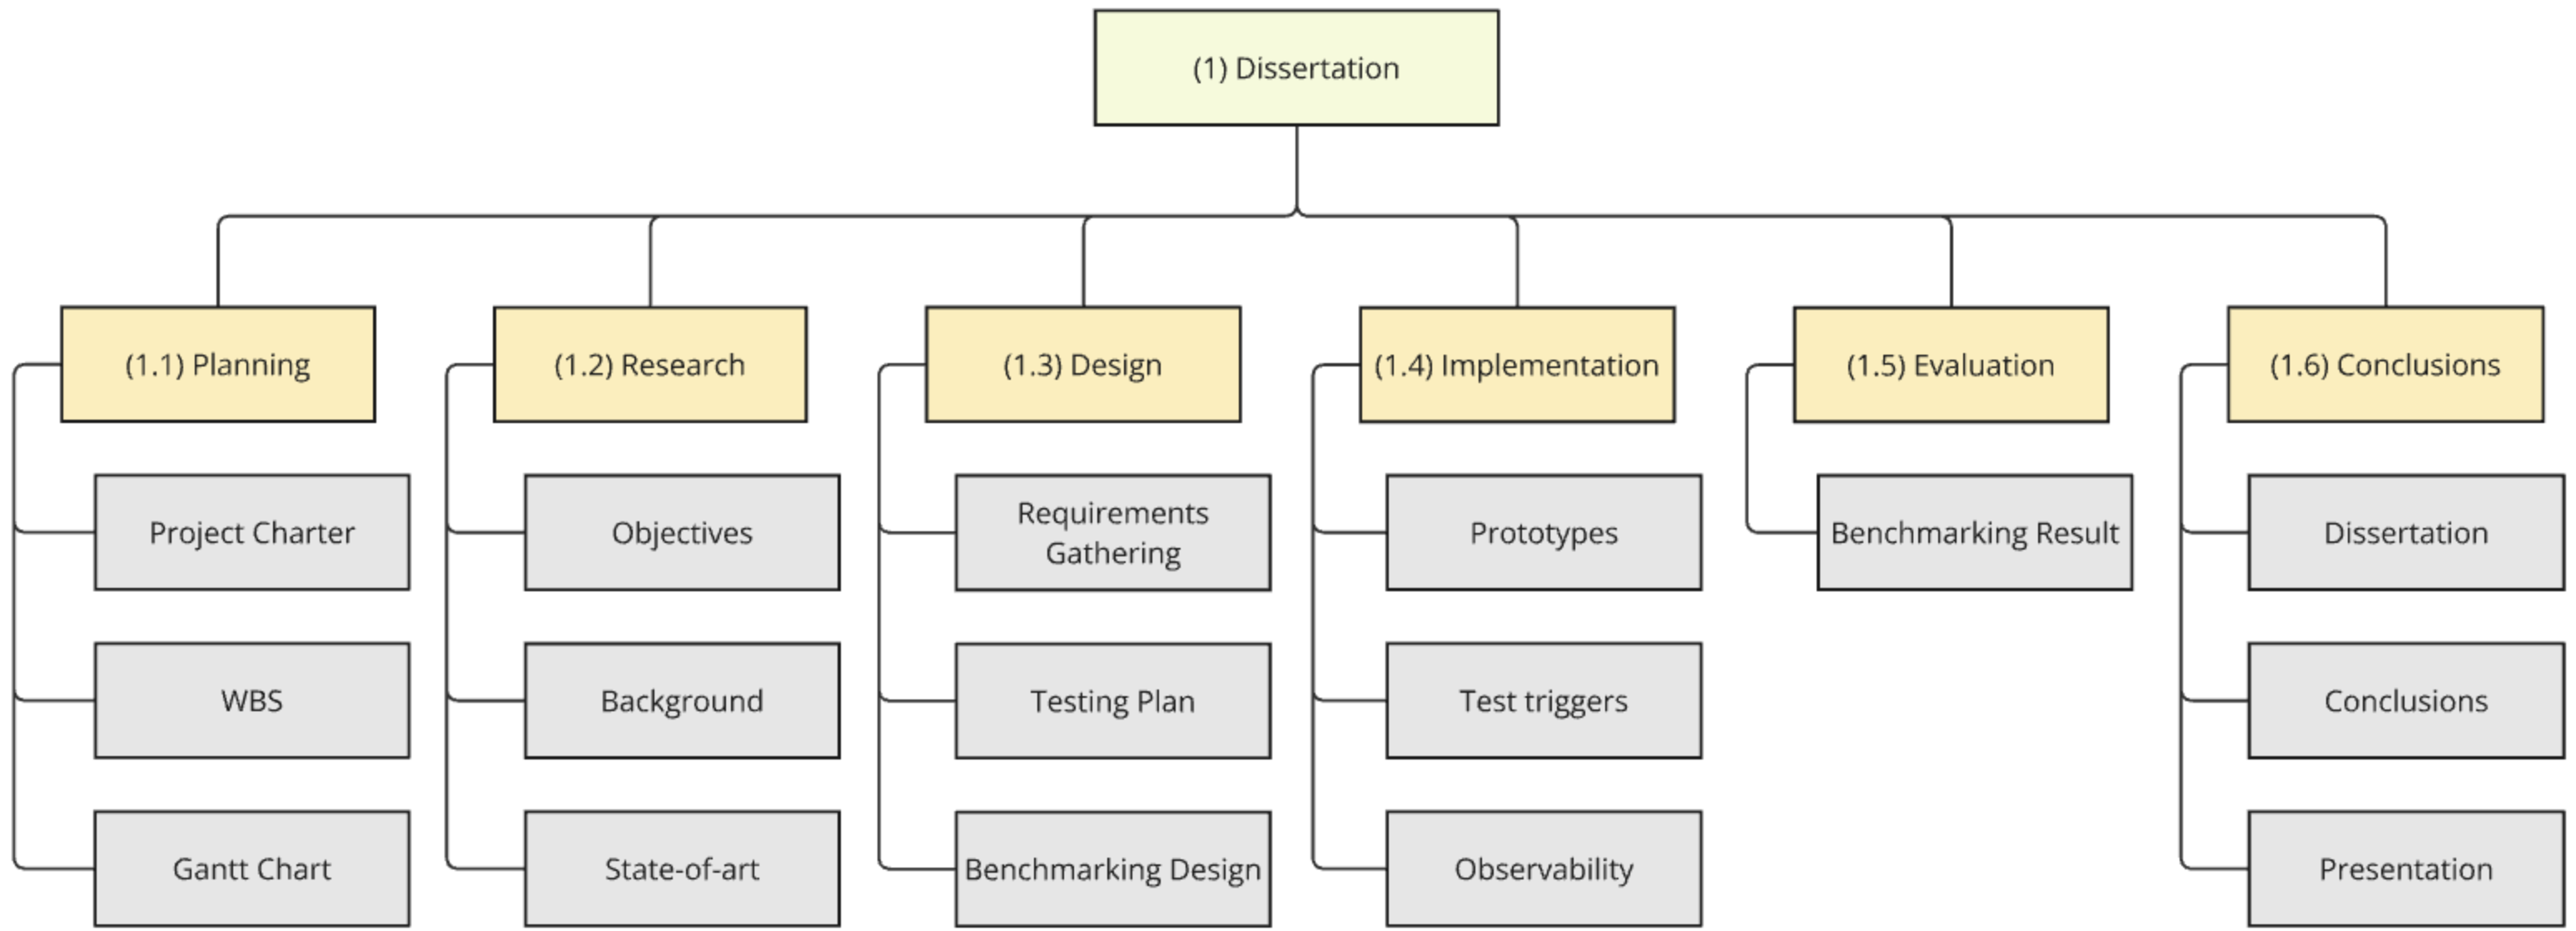
\includegraphics[width=\linewidth]{ch-planning/assets/wbs.png}
    \caption{The \gls{WBS} of the project.}
    \label{fig:wbs}
\end{figure}


\textbf{Work Breakdown Structure Dictionary} Following is described the \gls{WBS} Dictionary that as the responsibility of detailing each phase in order to be defined what are the goals and the acceptance criteria in a concise and clear way.

\begin{longtable}{|p{3cm}|p{2.5cm}|p{8cm}|}
    \hline
    \textbf{Item Name}             & \textbf{Type of Item} & \textbf{Additional Description / Acceptance Criteria}                                                                                                                                                                                                                                                                                                     \\ \hline
    \endfirsthead
    \hline
    \textbf{Item Name}             & \textbf{Type of Item} & \textbf{Additional Description / Acceptance Criteria}                                                                                                                                                                                                                                                                                                     \\ \hline
    \endhead
    (1.1) Planning                 & Phase                 & This phase includes all initial project setup tasks.                                                                                                                                                                                                                                                                                                      \\ \hline
    (1.1.1) Project Charter        & Deliverable           & The project charter must be created following the project's scope and management guidelines. \newline \textbf{Acceptance Criteria:} The project charter must be approved by the supervisor.                                                                                                                                                               \\ \hline
    (1.1.2) \gls{WBS}              & Deliverable           & The \gls{WBS} should break down the project into manageable components. \newline \textbf{Acceptance Criteria:} The WBS should be validated by the supervisor and include all project elements.                                                                                                                                                            \\ \hline
    (1.1.3) Gantt Chart            & Deliverable           & A detailed timeline outlining tasks, dependencies, action plan, milestones, and the dissertation deadline. \newline \textbf{Acceptance Criteria:} The Gantt chart must accurately reflect project phases and be reviewed by the supervisor.                                                                                                               \\ \hline
    \hline % Separator between phases

    (1.2) Research                 & Phase                 & This phase focuses on gathering the required knowledge and literature to support the project.                                                                                                                                                                                                                                                             \\ \hline
    (1.2.1) Objectives             & Deliverable           & Clear objectives for the project, that must detail what are the excepted outcomes. \newline \textbf{Acceptance Criteria:} Objectives should align with the research goals and be validated by the supervisor.                                                                                                                                             \\ \hline
    (1.2.2) Background             & Deliverable           & Research and summarize the background of fault tolerance in distributed systems and the distributed and concurrent programming languages.  \newline \textbf{Acceptance Criteria:} The background section should include sufficient theoretical content approved by the supervisor, and must include a clear justification for the languages chosen.       \\ \hline
    (1.2.3) State-of-art           & Deliverable           & Review the current literature on fault tolerance in Elixir, Go, and Scala with Akka. Also, what are the latest techniques for benchmarking distributed and concurrent programming, and if there are already studies on this topic. \newline \textbf{Acceptance Criteria:} State-of-the-art review must highlight gaps and relevance to the project scope. \\ \hline
    \hline % Separator between phases

    (1.3) Design                   & Phase                 & This phase involves requirements gathering, testing plan, and benchmarking design.                                                                                                                                                                                                                                                                        \\ \hline
    (1.3.1) Requirements Gathering & Deliverable           & Collect requirements for the benchmarking and evaluation of fault tolerance aspects. \newline \textbf{Acceptance Criteria:} Requirements must be detailed, reviewed, and approved by the supervisor.                                                                                                                                                      \\ \hline
    (1.3.2) Testing Plan           & Deliverable           & A plan for testing different fault tolerance strategies and mechanisms in Elixir, Go, and Scala with Akka. \newline \textbf{Acceptance Criteria:} Testing plan must include scenarios and validation methods, reviewed by the supervisor.                                                                                                                 \\ \hline
    (1.3.3) Benchmarking Design    & Deliverable           & Define the design for benchmarking environments. \newline \textbf{Acceptance Criteria:} Benchmarking environments design must be validated by the supervisor, and must adhere to the test plan created.                                                                                                                                                   \\ \hline
    \hline % Separator between phases

    (1.4) Implementation           & Phase                 & This phase involves the development of benchmarking prototypes.                                                                                                                                                                                                                                                                                           \\ \hline
    (1.4.1) Prototypes             & Deliverable           & Develop prototypes in Elixir, Go, and Scala with Akka for fault tolerance testing. \newline \textbf{Acceptance Criteria:} Prototypes must meet the test plan previously created and must be supported on the benchmarking design planned.                                                                                                                 \\ \hline
    (1.4.2) Test Triggers          & Deliverable           & Create fault injection mechanisms for testing fault tolerance. \newline \textbf{Acceptance Criteria:} Fault injection methods must simulate real-world scenarios and be validated by tests.                                                                                                                                                               \\ \hline
    (1.4.3) Observability          & Deliverable           & Implement observability tools for monitoring system behavior during tests. \newline \textbf{Acceptance Criteria:} Observability setup must capture the metrics defined on the test validations methods.                                                                                                                                                   \\ \hline
    \hline % Separator between phases

    (1.5) Evaluation               & Phase                 & Evaluate the results of the benchmarking tests.                                                                                                                                                                                                                                                                                                           \\ \hline
    (1.5.1) Benchmarking Result    & Deliverable           & Analyze and document the outcomes of benchmarking fault tolerance aspects. \newline \textbf{Acceptance Criteria:} Results must be clear, reproducible, and reviewed by the supervisor.                                                                                                                                                                    \\ \hline
    \hline % Separator between phases

    (1.6) Conclusions              & Phase                 & Finalize and present the results of the dissertation.                                                                                                                                                                                                                                                                                                     \\ \hline
    (1.6.1) Dissertation           & Deliverable           & Compile the dissertation document with findings and analyses. \newline \textbf{Acceptance Criteria:} Dissertation must meet university formatting and content guidelines.                                                                                                                                                                                 \\ \hline
    (1.6.2) Conclusions            & Deliverable           & Write concise conclusions summarizing key findings from the research, with the goal of creating a guide for future developers consult. \newline \textbf{Acceptance Criteria:} Conclusions must be concise and detail what are the cons and pros of using each language for each specific case, so that develops can easily decide.                        \\ \hline
    (1.6.3) Presentation           & Deliverable           & Prepare and deliver the final presentation to the evaluation committee. \newline \textbf{Acceptance Criteria:} Presentation must be clear and precise.                                                                                                                                                                                                    \\ \hline
\end{longtable}

\begin{comment}

\textbf{Item Name: (1.1) Planning} \\
\textbf{Type of Item:} Phase \\
\textbf{Description/Acceptance Criteria:} This phase includes initial project setup tasks. \\[0.5em]

\hspace{10mm} \textbf{Item Name: (1.1.1) Project Charter} \\
\hspace{10mm} \textbf{Type of Item:} Deliverable \\
\hspace{10mm} \textbf{Description/Acceptance Criteria:} The project charter must be created following the project's scope and management guidelines. \textbf{Acceptance Criteria:} It must be approved by the supervisor. \\[0.5em]

\textbf{Item Name: (1.1.2) WBS} \\
\textbf{Type of Item:} Deliverable \\
\textbf{Description/Acceptance Criteria:} Break down the project into manageable components using best practices. \textbf{Acceptance Criteria:} It must be validated by the supervisor and include all project elements. \\[0.5em]

\textbf{Item Name: (1.1.3) Gantt Chart} \\
\textbf{Type of Item:} Deliverable \\
\textbf{Description/Acceptance Criteria:} Create a detailed timeline outlining tasks, dependencies, and milestones. \textbf{Acceptance Criteria:} It must reflect project phases and be reviewed by the supervisor. \\[0.5em]

\textbf{Item Name: (1.2) Research} \\
\textbf{Type of Item:} Phase \\
\textbf{Description/Acceptance Criteria:} Focus on gathering required knowledge and literature for the project. \\[0.5em]

\textbf{Item Name: (1.2.1) Objectives} \\
\textbf{Type of Item:} Deliverable \\
\textbf{Description/Acceptance Criteria:} Define clear objectives for the comparison of fault tolerance in Elixir, Go, and Akka. \textbf{Acceptance Criteria:} Objectives must align with research goals and be validated by the supervisor. \\[0.5em]

\textbf{Item Name: (1.2.2) Background} \\
\textbf{Type of Item:} Deliverable \\
\textbf{Description/Acceptance Criteria:} Research and summarize the theoretical background of fault tolerance in distributed systems. \textbf{Acceptance Criteria:} It must cover sufficient depth and breadth and be approved by the supervisor. \\[0.5em]

\textbf{Item Name: (1.2.3) State-of-art} \\
\textbf{Type of Item:} Deliverable \\
\textbf{Description/Acceptance Criteria:} Review current literature on fault tolerance in Elixir, Go, and Akka. \textbf{Acceptance Criteria:} Must highlight gaps and relevance to the project scope. \\[0.5em]

\textbf{Item Name: (1.3) Design} \\
\textbf{Type of Item:} Phase \\
\textbf{Description/Acceptance Criteria:} Includes requirements gathering, testing plan, and benchmarking design. \\[0.5em]

\textbf{Item Name: (1.3.1) Requirements Gathering} \\
\textbf{Type of Item:} Deliverable \\
\textbf{Description/Acceptance Criteria:} Collect requirements for benchmarking and evaluating fault tolerance aspects. \textbf{Acceptance Criteria:} Requirements must be detailed, reviewed, and approved by the supervisor. \\[0.5em]

\textbf{Item Name: (1.3.2) Testing Plan} \\
\textbf{Type of Item:} Deliverable \\
\textbf{Description/Acceptance Criteria:} Plan for testing fault tolerance mechanisms in Elixir, Go, and Akka. \textbf{Acceptance Criteria:} The plan must include scenarios and validation methods, reviewed by the supervisor. \\[0.5em]

\textbf{Item Name: (1.3.3) Benchmarking Design} \\
\textbf{Type of Item:} Deliverable \\
\textbf{Description/Acceptance Criteria:} Define the methodology for benchmarking fault tolerance. \textbf{Acceptance Criteria:} It must be clear and validated by the supervisor. \\[0.5em]

\textbf{Item Name: (1.4) Implementation} \\
\textbf{Type of Item:} Phase \\
\textbf{Description/Acceptance Criteria:} Involves the development and deployment of benchmarking prototypes. \\[0.5em]

\textbf{Item Name: (1.4.1) Prototypes} \\
\textbf{Type of Item:} Deliverable \\
\textbf{Description/Acceptance Criteria:} Develop prototypes in Elixir, Go, and Akka for fault tolerance testing. \textbf{Acceptance Criteria:} Prototypes must meet design specifications and function as intended. \\[0.5em]

\textbf{Item Name: (1.4.2) Test Triggers} \\
\textbf{Type of Item:} Deliverable \\
\textbf{Description/Acceptance Criteria:} Create fault injection mechanisms for testing fault tolerance. \textbf{Acceptance Criteria:} Fault injection methods must simulate real-world scenarios and be validated by tests. \\[0.5em]

\textbf{Item Name: (1.4.3) Observability} \\
\textbf{Type of Item:} Deliverable \\
\textbf{Description/Acceptance Criteria:} Implement observability tools for monitoring system behavior during tests. \textbf{Acceptance Criteria:} The setup must capture necessary metrics and be validated. \\[0.5em]

\textbf{Item Name: (1.5) Evaluation} \\
\textbf{Type of Item:} Phase \\
\textbf{Description/Acceptance Criteria:} Evaluate results from benchmarking tests. \\[0.5em]

\textbf{Item Name: (1.5.1) Benchmarking Result} \\
\textbf{Type of Item:} Deliverable \\
\textbf{Description/Acceptance Criteria:} Analyze and document outcomes of benchmarking fault tolerance. \textbf{Acceptance Criteria:} Results must be clear, reproducible, and reviewed by the supervisor. \\[0.5em]

\textbf{Item Name: (1.6) Conclusions} \\
\textbf{Type of Item:} Phase \\
\textbf{Description/Acceptance Criteria:} Finalize and present the dissertation results. \\[0.5em]

\textbf{Item Name: (1.6.1) Dissertation} \\
\textbf{Type of Item:} Deliverable \\
\textbf{Description/Acceptance Criteria:} Compile the dissertation with findings and analyses. \textbf{Acceptance Criteria:} Must meet university formatting and content guidelines. \\[0.5em]

\textbf{Item Name: (1.6.2) Conclusions} \\
\textbf{Type of Item:} Deliverable \\
\textbf{Description/Acceptance Criteria:} Write conclusions summarizing key insights from the research. \textbf{Acceptance Criteria:} Must align with research objectives and supervisor feedback. \\[0.5em]

\textbf{Item Name: (1.6.3) Presentation} \\
\textbf{Type of Item:} Deliverable \\
\textbf{Description/Acceptance Criteria:} Prepare and deliver the final presentation to the evaluation committee. \textbf{Acceptance Criteria:} Presentation must be clear, engaging, and adhere to the allocated time. \\[0.5em]
\end{comment}

\section{Gantt Diagram}

\section{Risk Management}

